\documentclass[aspectratio=169]{beamer}

% Default packages
\usepackage[T1]{fontenc}
\usepackage[utf8]{inputenc}
\usepackage[english]{babel}
\usepackage{pgfplots}
\pgfplotsset{compat=newest}
\usepackage{booktabs}
\usepackage{siunitx}
\usepackage[backend=biber,
            style=alphabetic,
            %backref=true,
            abbreviate=false,
            dateabbrev=false,
            alldates=long]{biblatex}

\addbibresource{bibliography.bib}
\usepackage{minted} % python code

% Font selection
% Latin Modern
\usepackage{lmodern}
% Verdana font type
%\usepackage{verdana}
% Helvetica
%\usepackage{helvet}
% Times (text and math)
%\usepackage{newtx, newtxmath}
% Nice font combination
%\usepackage{mathptmx} % math
%\usepackage{sourcesanspro} % sans-serif
\usepackage{charter} % serif

% Use DTU theme, see below for options
\usetheme[department=compute]{DTU}

\title[Master's Thesis]{A Flutter Package for Real-Time Mobility Feature
Computation}
\author{Thomas Nygaard Nilsson, s144470}
\institute{Master's Thesis Defense}
\date{\today}
	
\newcommand{\tabitem}{{\color{dtured}$\bullet$} }

\begin{document}
\frame{
	\maketitle
}

\frame{
	\frametitle{Background}
	\begin{itemize}
		\item Depression
		\item Treated with therapy or medication
		\item Behavioural activation
		\item Relies on self-reporting (subjective data)
	\end{itemize}
}

\frame{
	\frametitle{Mobile Sensing}
	\begin{itemize}
	    \item Infer user state from objective sensor data
		\item Can include many data channels (ECG, Steps, Sleep etc)
		\item Location data is very common for depression-related mobile sensing \cite{objective_smartphone_data_as_diagnostic_marker, extraction-of-behavioural-features, palmius2017, Saeb2015} 
	\end{itemize}
}

\frame{
	\frametitle{Mobility Features}
	\begin{itemize}
		\item Features derived from location data over time
		\item Capture the user’s ‘mobility’ patterns
		\item Correlated with self-reported behaviour and mental state \cite{Saeb2015, Canzian2015, palmius2017}
	\end{itemize}
}

\frame{
	\frametitle{Problem Statement}

	\begin{itemize}
		\item Existing contributions are hard to reproduce (source code)
        \item Algorithms are 'off-line'
        \item Real-time: Any time of the day, on the device, fast
        \item Solution: Software package for mobile health researchers (programmers)
	\end{itemize}
			\begin{figure}
	    \centering
	    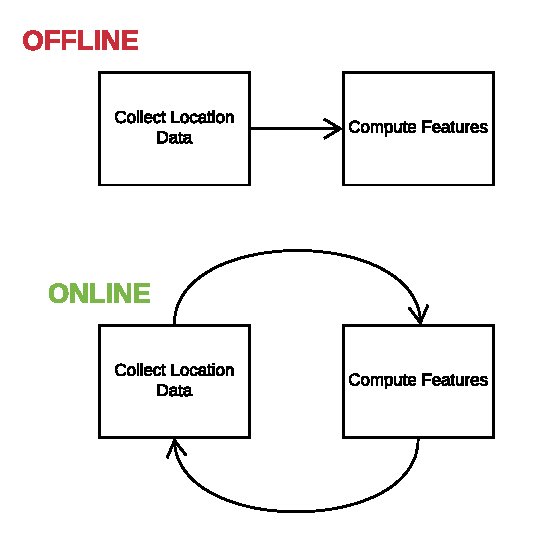
\includegraphics[width=0.35\textwidth]{study-offline-online.pdf}
	\end{figure}

}

\frame{
	\frametitle{Research Questions}
	\begin{itemize}
    \item Which mobility features are relevant to include in a software package? 
    \item How can these features be computed in real-time, on a smartphone device?
    \item How does the design of such a software package look like?
	\end{itemize}
}


% https://pub.dev/packages/mobility_features

\frame{
	\frametitle{Which mobility features are relevant to include in a software package?}
	\begin{itemize}
    \item Stops, Places, Moves
    \item Number of Places
    \item Home Stay
    \item Entropy/Normalized Entropy
    \item Distance Travelled
    \item Location Variance
    \item Routine Index\footnote{Not the same implementation as in the literature}
    \item Based on the work of Saeb, Cuttone and Canzian et al. to a large degree \cite{Saeb2015, sparse-location-2014, Canzian2015} 
    
	\end{itemize}
}

\frame{
	\frametitle{How can these features be computed in real-time, on a smartphone device?}
	\begin{itemize}
    \item Re-define feature algorithms st. they work with an incomplete dataset
    \item Routine Index requires historical data (stops)
    \item Solution: Store stops and moves on disk
    \item Implemented in the Flutter framework (Dart programming language)
	\end{itemize}
}

\frame{
	\frametitle{How does the design of such a software package look like?}
	\begin{itemize}
    \item Features computed with 3 lines of Dart code
    \begin{itemize}
        \item Programming interface hides the implementation from the programmer
        \item Makes it easier to use
    \end{itemize}
    
    \item Location data collection done via a separate plugin
    \begin{itemize}
        \item Gives programmer flexibility
        \item Dependency issues avoided
        \item Package maintenance much easier
    \end{itemize}
   
	\end{itemize}
}


\frame{
	\frametitle{How can these features be computed in real-time, on a smartphone device?}
	\begin{itemize}
    \item Re-define feature algorithms st. they work with an incomplete dataset
    \item Routine Index requires historical data (stops)
    \item Solution: Store stops and moves on disk
    \item Implemented in the Flutter framework (Dart programming language)
	\end{itemize}
}

\frame{
	\frametitle{Field Study}
	\begin{itemize}
    \item 10 participants, 3 weeks
    \item Features computed daily from location data
    \item Subjective answers collected daily
    \item 3 features evaluated (Number of Places, Home Stay, Routine Index)
	\end{itemize}
	\begin{table}[]
    \centering
    \begin{tabular}{|l|l|l|l|}
    \hline
                        & \textbf{Number of Places} & \textbf{Home Stay} & \textbf{Routine Index} \\ \hline
    \textbf{Mean RMSE}       & 0.99                      & 14.27 (\%)         & 22.5 (\%)              \\ \hline
    \end{tabular}
    \caption{The mean RMSE computed for all participants}
    \label{tab:error-table}
\end{table}
}

% -- API

\frame{
	\frametitle{Package Usage}
	\begin{figure}[h]
    \centering
    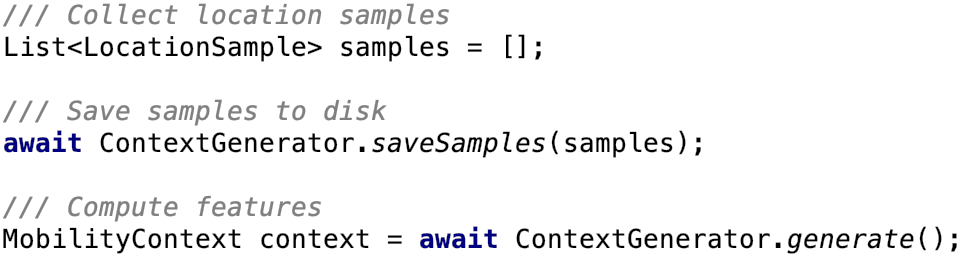
\includegraphics[width=0.5\textwidth]{code-example.png}
    \caption{All the three lines of code necessary for the application developer to write}
    \label{fig:code-example-intro}
\end{figure}
}


% ----- Conclusion/Future Work



\frame{
	\frametitle{Limitations}
	\begin{itemize}
    \item Handles missing data poorly 
    \begin{itemize}
        \item Implement imputation
        \item May bias the Routine Index, but is a better alternative
    \end{itemize}
    
    \item Routine Index has been redefined but not clinically evaluated
    
    \item Feature computation procedure
    \begin{itemize}
        \item Async computation
        \item Daily computation
    \end{itemize}

	\end{itemize}
}

\frame{
	\frametitle{Future Work}
	\begin{itemize}
    \item CAMS integration
    \item MUBS
    \begin{itemize}
        \item Give recommendations based on features
        \item Use features to improve the recommender algorithm
    \end{itemize}
	\end{itemize}
}


\frame{
	\frametitle{Conclusion}
	\begin{itemize}
    \item Package is released at \url{https://pub.dev/packages/mobility_features}
    \item Programmer can compute features with 3 lines of code
    \item 
    \item 
	\end{itemize}
}

% \frame{
% 	\frametitle{}
% 	\begin{itemize}
%     \item 
%     \item 
%     \item 
%     \item 
% 	\end{itemize}
% }

 



% \frame{
% 	\frametitle{Outline}
% 	\tableofcontents
% }

% \section{User Guide}

% \subsection{Package Options}
% \frame[allowframebreaks]{
% 	\frametitle{Package Options}
% 	\begin{block}{[department=]}
% 		\begin{tabular}{ll}
% 			\tabitem aqua & DTU Aqua\\ 
% 			\tabitem byg & DTU Civil Engineering\\
% 			\tabitem compute & DTU Compute\\
% 			\tabitem elektro & DTU Electrical Engineering\\
% 			\tabitem energikonvertering & DTU Energy Conversion\\
% 			\tabitem fotonik & DTU Fotonik\\
% 			\tabitem fysik & DTU Physics\\
% 			\tabitem food & DTU Food\\
% 			\tabitem kemi & DTU Chemistry\\
% 			\tabitem kemiteknik & DTU Chemical Engineering
% 		\end{tabular}
% 	\end{block}
	
% 	\begin{block}{[department=]}
% 		\begin{tabular}{ll}
% 			\tabitem management & DTU Management Engineering\\
% 			\tabitem mekanik & DTU Mechanical Engineering\\
% 			\tabitem miljo & DTU Environment Engineering\\
% 			\tabitem nanotek & DTU Nanotech\\
% 			\tabitem space & DTU Space\\ 
% 			\tabitem systembiologi & DTU Systems Biology\\
% 			\tabitem transport & DTU Transport\\
% 			\tabitem vaterinaerinstituttet & DTU Vet\\
% 			\tabitem vindenergi & DTU Wind Energy
% 		\end{tabular}
% 	\end{block}
	
% 	\begin{block}{[showsection=]}
% 		\begin{tabular}{ll}
% 			\tabitem false & Remove section from above frame title\\
% 			\tabitem true (default) & Display section above frame title
% 		\end{tabular}
% 	\end{block}
% }

% \subsection{Date Format}
% \frame{
% 	\frametitle{Date Format}
% 	\begin{block}{Default Date Format}
% 		\texttt{[Numeric]Day.[Numeric]Month.[Numeric]Year}
% 	\end{block}
	
% 	\begin{block}{Customize Date Format}
% 		Place the following code snippet in the preamble:
% 		\texttt{\textbackslash newdateformat\{myDateFormat\}\{\textbackslash THEDAY-\textbackslash THEMONTH-\textbackslash THEYEAR\}}
% 		\texttt{\textbackslash renewcommand\{\textbackslash DTUDateFormat\}\{\textbackslash myDateFormat\}}
% 	\end{block}
% }



% \section{Demonstration}

% \subsection{Lists}
% \frame{
% 	\frametitle{Lists}
% 	\begin{itemize}
% 		\item Notice
% 		\item the
% 		\item red
% 		\item bullet
% 	\end{itemize}
	
% 	\begin{enumerate}
% 		\item Wow
% 		\item numbered
% 		\item list
% 	\end{enumerate}
% }

% \subsection{Blocks}
% \frame{
% 	\frametitle{Blocks}
% 	\begin{block}{Cool block}
% 		Get nice visual effects by organizing content into \textbf{blocks}. Title background color matches the red from DTU logo.
% 	\end{block}
% }

% \subsection{Tables}
% \frame{
% 	\frametitle{Tables}
% 	\begin{table}
% 		\small
% 		\caption{Not a regular table. Content is aligned with respect to the decimal symbol.}
% 		\label{tab:S:standard}
% 		\centering
% 		\begin{tabular}{S}
% 			\toprule
% 			{Some Values} \\
% 			\midrule
% 			2.3456 \\
% 			34.2345 \\
% 			-6.7835 \\
% 			90.473 \\
% 			5642.5 \\
% 			1.2e3 \\
% 			e4 \\
% 			\bottomrule
% 		\end{tabular}
% 	\end{table}
% }

% \subsection{Plots}
% \frame{
% 	\frametitle{Plots}
% 	Stunt your colleagues with amazing plots (pgfplots).
% 	\begin{figure}[htbp]
% 	\centering
% 	\small
% 	\begin{tikzpicture}
% 		\begin{axis}[
% 			width=0.4\textwidth,
% 			grid=major,
% 			title={Model Validation},
% 			xlabel={X},
% 			ylabel={Y}
% 		]
		
% 		\addplot {-x^5 - 242};
% 		\addlegendentry{model}
	
% 		\addplot coordinates {
% 			(-4.77778,2027.60977)
% 			(-3.55556,347.84069)
% 			(-2.33333,22.58953)
% 			(-1.11111,-493.50066)
% 			(0.11111,46.66082)
% 			(1.33333,-205.56286)
% 			(2.55556,-341.40638)
% 			(3.77778,-1169.24780)
% 			(5.00000,-3269.56775)
% 		};
% 		\addlegendentry{estimate}
% 		\end{axis}
% 	\end{tikzpicture}
% 	\end{figure}
% }

% \subsection{Frame Numbers}
% \frame{
% 	\frametitle{Frame number instead of page number}
% 	\setbeamercovered{transparent}
% 	\begin{itemize}
% 		\item<1-> Watch the frame number.
% 		\item<2-> It doesn't change!
% 	\end{itemize}
% }

% {
% \setbeamercolor{background canvas}{bg=black} % Background color
% 	\frame[dtuwhitelogo]{
% 		\frametitle{Hello Blackness}
% 		Here is another frame style!
% 	}
% }

% \section{Final Remarks}

% \subsection{Fonts}
% \frame{
% 	\frametitle{Fonts}
% 	\begin{itemize}
% 		\item You can set whatever font you like in the preamble. E.g.:
% 		\begin{itemize}
% 			\item \texttt{\textbackslash usepackage\{lmodern\} \% Latin Modern}
% 			\item \texttt{\textbackslash usepackage\{helvet\} \% Helvetica}
% 			\item \texttt{\textbackslash usepackage\{verdana\} \% Verdana}
% 			\item \texttt{\textbackslash usepackage\{newtx, newtxmath\} \% Times (text and math)}
% 		\end{itemize}
		
% 		\item DTU recommends Verdana but this font type is not available by default on all operating systems:
% 		\begin{itemize}
% 			\item Windows: include the \texttt{verdana} package in the preamble and MiKTeX will do the rest;
% 			\item Linux and OS X: before including the \texttt{verdana} package in your preamble, run the \texttt{install\_fonts.sh} script from our package.
% 		\end{itemize}
% 	\end{itemize}
% }

% %================================================
% %===  Define the contact details
% \newcommand\contactTable{ %
%   \begin{tabular}{lr}
%     \multicolumn{2}{l}{Your Name} \\ 
%     \multicolumn{2}{l}{\LaTeX\ Support Group, Technical University of Denmark (DTU)} \\ \midrule
%     Building 308, Room 119    & latex-support@student.dtu.dk. \\
%     2800 Kgs. Lyngby, Denmark & +45 4525 phone \\
%     http://www.latex.dtu.dk   & +45 4525 fax
%   \end{tabular}
% }%

% \frame[dtuwhitelogo, bgfilename=dtu_bg_fiber]{
%   \begin{tikzpicture}[remember picture,overlay]
%     \node[fill=black, fill opacity=0.9, 
%           text=white, text opacity=1.0,
%           rounded corners=5pt, 
%           font=\scriptsize] at (current page.center) {\contactTable};
%   \end{tikzpicture}
% }

% \frame[dtuwhitelogo, bgfilename=dtu_bg_nano]{
%   \begin{tikzpicture}[remember picture,overlay]
%     \node[fill=black, fill opacity=0.9, 
%           text=white, text opacity=1.0,
%           rounded corners=5pt, 
%           font=\scriptsize] at (current page.center) {\contactTable};
%   \end{tikzpicture}
% }

% \frame[dtuwhitelogo, bgfilename=dtu_bg_pink]{
%   \begin{tikzpicture}[remember picture,overlay]
%     \node[fill=white, fill opacity=0.8, 
%           text=black, text opacity=1.0,
%           rounded corners=5pt, 
%           font=\scriptsize] at (current page.center) {\contactTable};
%   \end{tikzpicture}
% }

% \frame{
% 	\frametitle{Contact}
	
% 	\begin{center}
% 		File bugs and feature requests at \url{http://gitlab.gbar.dtu.dk/latex/dtutemplates/issues}
% 	\end{center}
% }

% \frame[allowframebreaks]{
% 	\frametitle{Release History}
% 	\begin{block}{v1.12}
% 		\begin{itemize}
% 			\item Frame number instead of page number.
% 		\end{itemize}
% 	\end{block}
% 	\begin{block}{v1.11}
% 		\begin{itemize}
% 			\item Long titles are displayed correctly in the footer;
% 			\item Department logos have the correct RGB color;
% 			\item The aspect ratio of the slides can be changed using beamer options.
% 		\end{itemize}
% 	\end{block}
% 	\begin{block}{v1.1}
% 		\begin{itemize}
% 			\item Fonts options;
% 			\item Poster template;
% 			\item Frame backgrounds;
% 			\item Black frames with white logo;
% 			\item Address boxes.
% 		\end{itemize}
% 	\end{block}
% 	\begin{block}{v1.03}
% 		\begin{itemize}
% 			\item New logos for \texttt{vindenergi} and \texttt{kemiteknik}.
% 		\end{itemize}
% 	\end{block}
% 	\begin{block}{v1.02}
% 		\begin{itemize}
% 			\item Date format is now customizable.
% 		\end{itemize}
% 	\end{block}
% 	\begin{block}{v1.01}
% 		\begin{itemize}
% 			\item \texttt{dtuletter} template included;
% 			\item Package name changed to \texttt{dtutemplates}.
% 		\end{itemize}
% 	\end{block}
% }
\end{document}